
\chapter{ Cadre du projet }
\clearpage
\section*{Introduction }
Après une mise en contexte de notre projet, nous passerons à détailler sa méthodologie de développement.
\`A ce niveau, une question devient ligitime : pourquoi sommes nous dans l'obligation de détailler notre méthodologie de développement de ce projet déjà ?
La réponse est simple mais méliorative : nous faisons face à un cahier de charges dynamique dont les contraintes peuvent subir des changements significatifs tout le long du projet. 
De ce fait, nous ne sommes pas dans un processus de développement classique, waterfall, connu par la succession des étapes collecte des besoins, conception et réalisation \cite{SoftwareEngeneering1}.
En génie logiciel, ce type de cahier de charges dynamique doit être traité avec précautions.
La méthodologie de développement d'un tel cahier de charges doit respecter un processus de développement à la fois itératif et incrémental \cite{SoftwareEngeneering3,SoftwareEngeneering2}.
La deuxième section de ce chapitre apporte plus d'appui au choix de la méthodologie de développement à adopter dans notre situation.
La conception des systèmes mécatroniques suit le langage de modélisation SysML (System Modeling Language). Qui est le langage de modélisation universel lors de la modélisation des systèmes mécatroniques \corrg{ \cite{Hal}}. C'est pourquoi nous exploiterons les diagrammes des exigences et des cas d'utilisation afin de présenter notre cahier de charges final dans la dernière section de ce chapitre.

\section{Problématique }
Depuis des temps immémoriaux, l'agriculture était très importante dans la mesure où elle faisait partie intégrante de la vie humaine et demeure d'une grande importance économique et sociopolitique du fait de sa contribution à la réalisation des objectifs nationaux en matière de sécurité alimentaire, de création de revenus, d'emplois, d'équilibre régional et de gestion des ressources naturelles. Néanmoins ce secteur central a étalé une faiblesse importante mondiale et régionale de compétitivité sur les marchés nationaux et internationaux suite à un manque de la technique et de l'innovation qui reflète une faible production et l'absence de qualité des produits agricoles d'organisations professionnelles bien développée. Les agriculteurs doivent constamment faire des miracles pour trouver des solutions à de nouveaux problèmes. Les défis à relever à l'avenir peuvent être très différents des problèmes rencontrés aujourd'hui. Pour cette raison-là, l'agriculture a connu de nombreuses crises vue qu'elle utilise les mêmes moyens sans innover de nouvelles technologies ni augmenter sa productivité.

Ces dernières années, le monde a été confronté à une baisse importante de la production agricole. Par exemple, au Brésil, le premier producteur d'oranges dans le monde avec plus de 19 millions de tonnes d'où proviennent plus de la moitié des fruits utilisés pour fabriquer les jus consommés à travers le monde. D'après les estimations du département américain de l'Agriculture (Usda), la situation est particulièrement critique vu que la production d'oranges risque d'être la plus faible depuis plus de vingt ans. En Tunisie, la production d'agrumes de la campagne 2017/2018 a fortement chuté à 38,2 \%, soit 346 000 tonnes \cite{onagri2017/2018}.

En plus, récemment à cause de cette crise sanitaire dûe au covid19, le secteur agricole rencontre d'autres problèmes et d'autres challenges. Il a perturbé le fonctionnement de l'agriculture et du système alimentaire dans son processus de production menant au centre de consommation. En raison des restrictions, il n'y a moins de travailleurs et des ouvriers dans de nombreux secteurs et domaines, ce qui peut facilement affecter la production et les économies mondiales et régionales. Le confinement des pays et la fermeture des frontières ont une forte incidence sur la rapidité et la flexibilité du modèle agricole. Il y'a donc moins d'innovations alternatives ce qui peut refléter un ralentissement de la production agricole.

\section{Objectif }
L'objectif de notre projet de fin d'études est d'utiliser les nouvelles technologies pour améliorer les performances économiques et environnementales des productions agricoles. Afin de s'organiser de manière appropriée, les agriculteurs ont besoin d'anticiper leur production. Mais le comptage des fruits est une tâche qui prend beaucoup de temps. Notre projet nommé « AGRIDrone » est consacré à optimiser ce temps perdu par le développement d'un système automatisé intégré dans un drone pour le comptage des oranges sur l'arbre. 


Ce système va mettre au point une méthode de travail plus efficace et bien précis qui utilise l'intelligence artificielle pour permettre aux fournisseurs de produits agricoles d'optimiser leurs récoltes et de planifier leurs ventes sur le marché. La technologie des drones pourrait aider les agriculteurs du monde entier à surveiller la croissance de leurs cultures, lutter contre les nuisibles, et bien plus encore. Grâce à la caméra et aux capteurs embarqués, le drone peut mesurer de nombreux indicateurs de l'état et des besoins de la plante. En fait, notre système fournit des informations plus précises et une variété de données.

Bien que le prélèvement ait été exécuté manuellement, les informations recueillies par le drone permet aux agriculteurs d'identifier les zones à traiter, de déterminer l'intervention la plus appropriée et de réduire la quantité de traitement utilisée. Tout cela sera facile et nous fera gagner de temps non négligeable avec cette nouvelle innovation.



\section[Methodologie]{Méthodologie de gestion de projet }
Cette méthodologie nous permet d'analyser l'environnement de notre projet, d'appliquer des méthodes techniques et d'évaluer l'opportunité jusqu'à l'achèvement de notre travail.
\subsection{Choix de méthodologie }
Afin d'assurer le bon déroulement des différentes étapes dans notre projet, nous avons choisi la méthode Agile Scrum pour gérer notre travail, concevoir et développer nos systèmes pour des raisons claires. Ce processus  s'inscrit parfaitement dans la décomposition de notre projet qui s'appuie sur les avantages suivants :
\begin{itemize}
	\item[$\bullet$] Plus de flexibilité et de réactivité
	\item[$\bullet$] Traduire et organiser le projet de façon simple, transparente et pragmatique
\end{itemize}

\subsection{Présentation de la méthodologie scrum }
La méthodologie Scrum nous a aidé dans la gestion de notre travail en planifiant les tâches à réaliser durant notre projet. D'abord, nous préparons ces tâches. Puis, nous assistons à une réunion pendant 15 minutes afin de les sélectionner et démarrer un sprint. Ensuite, nous classifions dans un tableau agile les activités selon l'avancement de chacune (à faire, en cours, sprint review, sprint retrospective et fini). Finalement, nous fermons le sprint pour passer à un autre.
Il existe trois rôles principaux intervenant dans la méthode agile scrum:
\subsubsection{Product owner }
C'est la personne ayant la responsabilité de produire et de maintenir à jour le carnet de produit. Elle détermine les priorités et prend les décisions d'orientation du projet.
\subsubsection{Scrum master  }
Celui qui s’assure que les principes et valeurs du scrum sont
respectées et veille au bon déroulement et avancement du projet. De plus, il facilite la communication au sein de l’équipe ainsi qu'il cherche à améliorer la productivité et le savoir-faire de son équipe.
\subsubsection{L'équipe développement  }
Constituée généralement de 2 à 10 développeurs. Elle regroupe tous les rôles habituellement nécessaires à un projet tels que l'architecte, le concepteur, le développeur, le testeur,... Elle est « auto-organisée » et reste inchangée pendant toute la durée du sprint.

La figure \ref{fig:A.S} présente le déroulement de la gestion de projet par Scrum \cite{Crochet}.
\begin{figure} [H]
	\begin{center}
		\centering
		\vskip 1.5cm
		\hspace*{-0.5cm}
		\fbox{\includegraphics[width=0.75\linewidth]{Images/Méthode Scrum}}
	\end{center}
	\caption{\label{fig:A.S}Agile Scrum}
\end{figure}
\section{Analyse des besoins }	
L'analyse des besoins est une des premières techniques de gestion de projet à mettre en oeuvre.

Cette partie sera utilisée pour jeter les bases de la collecte des besoins du système avant d'être réalisée.
Dans le but de préciser les besoins des utilisateurs de notre système, nous présenterons les besoins fonctionnels ainsi que les besoins non fonctionnels.

\subsection{Les besoins fonctionnels}
Notre projet consiste à développer un drone qui doit survoler la parcelle tout en inspectant les arbres afin de détecter pour chaque arbre les oranges présentes.

Parmi les différents besoins fonctionnels de notre système, nous citons:
\begin{itemize}
	\item [$\bullet$] Le paramétrage du contrôleur de vol 
	\item [$\bullet$]La configuration de la radiocommande 
	\item [$\bullet$]Le contrôle de l'AGRIDrone
	\item[$\bullet$] La génération des rapports
\end{itemize} 

En plus, les besoins fonctionnels et les attentes vis-à-vis notre AGRIDrone varient d'un acteur à un autre. Pour celà, nous allons détailler le rôle de chaque acteur en se basant sur des diagrammes de cas d'utilisation \ref{Cas d'utilisation}.

\subsection{Les besoins non fonctionnels}
Après avoir cité les besoins fonctionnels, nous présentons
les besoins non fonctionnels de drone qui sont liés aux contraintes dont il faut tenir compte pour appliquer une solution adéquate et qui ont été définis tels que:
\begin{itemize}
	\item [$\bullet$] \textbf{La stabilité :}
	
	
	Dans le cadre de ce travail, le drone devra être stable, l'AGRIDrone doit être robuste en terme de repositionnement automatique aprés une perturbation.	
	\item [$\bullet$] \textbf{L'extensibilitè : }
	
	
	L'AGRIDrone doit permettre des nouvelles fonctionnalités.
	
	\item [$\bullet$] \textbf{La portée : } 
	
	
	On doit pouvoir contrôler le drone jusqu'à 500m.
	
	
	\item [$\bullet$] \textbf{La maintenabilité : }  
	
	Subir à une intervention de maintenance en terme de modifications et corrections des erreurs.
	\end {itemize}
	\section{Diagramme d'exigence }
	Après avoir étudié attentivement les besoins de  notre système, nous avons effectué sa modélisation à travers le diagramme d'exigence permettant de décrire graphiquement les capacités à réaliser et les contraintes qui doivent être dépassées.
	
	Une exigence comporte : 
	\begin{itemize}
		\item [$\bullet$] Un intitulé 
		
		\item [$\bullet$]Un texte descriptif 
		
		\item [$\bullet$]Un identifiant unique
	\end{itemize}
	
	\begin{figure}[H] 
		\begin{center} 
			\centering
			\vskip 1cm
			\hspace*{-1.3cm} 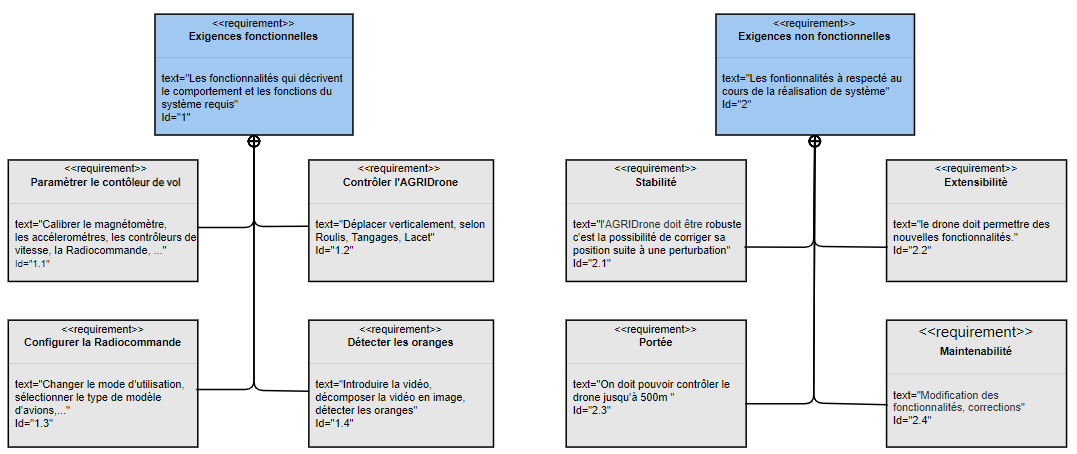
\includegraphics[width=1.2\linewidth]{Images/Diagramme d'exigence}
			\vskip 0.5cm
			\caption{Diagramme d'exigence}
		\end{center}
		\end {figure}
		
		
		\section{Diagrammes des cas d'utilisation }\label{Cas d'utilisation}
		
		Cette structure est bien adaptée pour décrire de manière claire les fonctions et les objectifs les plus importants d'un système. C'est pour cette raison que l'élaboration d'un diagramme de cas d'utilisation est souvent l'une des premières étapes lors de la conception de système ou de la planification de nouveaux processus métier. Cela permet de visualiser facilement et clairement quels cas d'utilisation doivent être pris en compte dans la conception pour que les acteurs atteignent les objectifs escomptés. 
		
		Nous illustrons dans la suite les principaux diagrammes de cas d'utilisation.
		\subsection{Cas d'utilisation global }
		Nous décrivons en tant qu'utilisateurs ce diagramme  qui donne un aperçu global sur le rôle de chaque acteur afin de comprendre l'idée générale du projet.
		
		
		\begin {figure} [H]
		\begin{center}
			\centering
			\hspace*{-1.1cm}\fbox{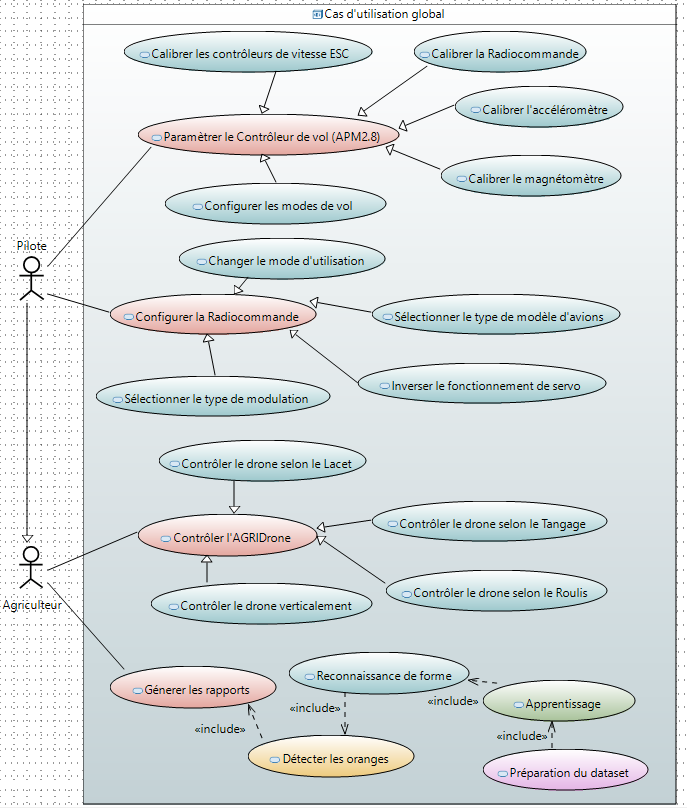
\includegraphics[width=1\linewidth]{Images/Diagramme de cas d'utilisation globale}}
		\end{center}
		
		\caption{Diagramme de cas d'utilisation global}
		\end {figure}
		
		Ci-dessous nous exposons quelques cas d'utilisation afin de mieux comprendre les caractéristiques contenues dans chaque cas.
		
		
		\subsection{Cas d'utilisation du Pilote}
		Nous montrons à travers la figure \ref{fig:D.P} le diagramme de cas d'utilisation du pilote qui permet de déterminer les principales fonctions qu'il doit effectuer. À savoir, en paramétrant le contôleur de vol, cet acteur a la possibilité de calibrer les contrôleurs de vitesses, la radiocommande, l'accéléromètre, le magnétomètre et régler les modes de vol. La deuxième tâche consiste à configurer la radiocommande d'où la possibilité de changer le mode d'utilisation, sélectionner le type de modèle d'avions, inverser les fonctionnements du servos et sélectionner le type de modulation. Le pilote doit aussi contrôler l'AGRIDrone en le déplaçant verticalement, selon le lacet, le tanguage et le roulis.
		\begin {figure}[H] 
		\begin{center} 
			\centering
			\hspace*{0.1cm}		\fbox{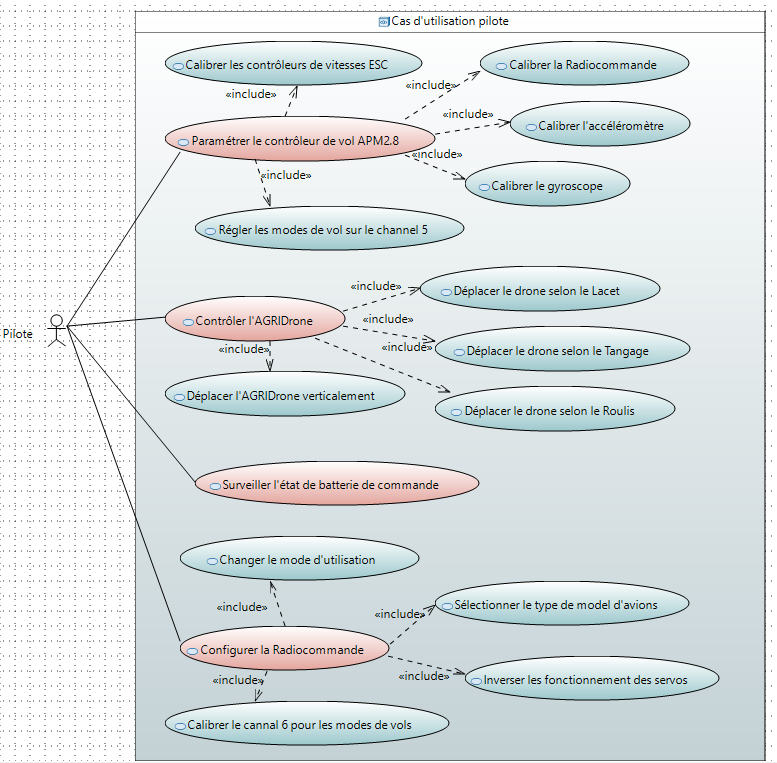
\includegraphics[width=0.8\linewidth]{Images/Diagramme de cas d'utilisation pilote}}
		\end{center}
		
		\caption{\label{fig:D.P}Diagramme de cas d'utilasation du pilote}
		\end {figure}
		
		
		\subsection{Cas d'utilisation de l'agriculteur }
		La figure \ref{fig:D.A} décrit le cas d'utilisation de l'agriculteur qui peut contrôler l'AGRIDrone avec les mêmes procédures que suit le pilote et générer les rapports après avoir détecter les oranges. Cette opération à son tour se produit à condition que la reconnaissance de forme s'établit. 
		\begin{figure}[H] 
			\begin{center} 
				\centering
				\hspace*{0cm}	\fbox{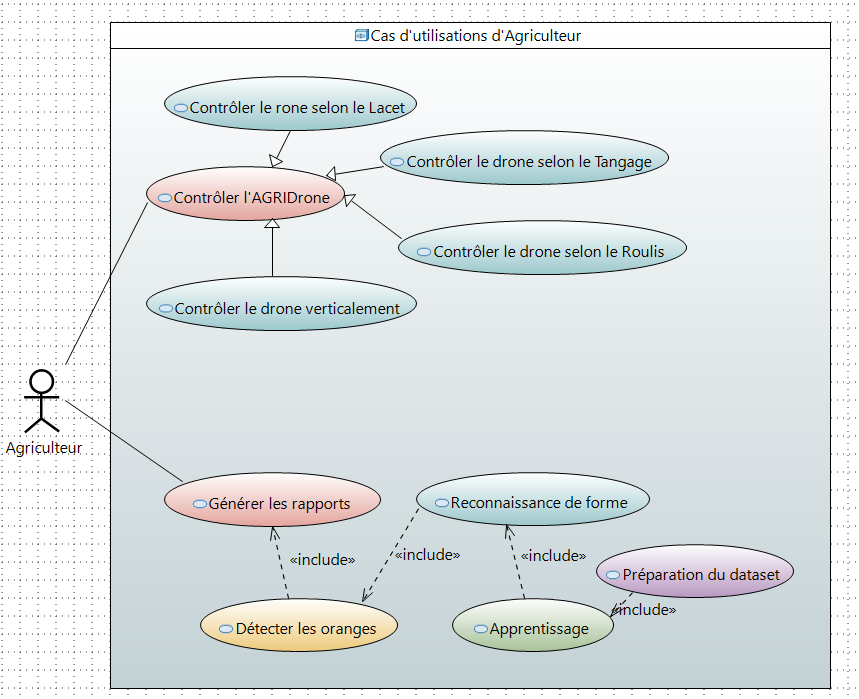
\includegraphics[width=0.9\linewidth]{Images/Diagramme de cas d'utilisation agriculture}}
			\end{center}
			
			\caption{\label{fig:D.A}Diagramme de cas d'utilisation de l'agriculteur}	
			
			\end {figure}
			
			\section*{Conclusion}
			Le long de ce chapitre, nous avons exposé la problématique à partir de laquelle nous avons créé l'objectif de notre projet et nous avons montré la phase de la méthodologie de travail, de la spécification des besoins et de la conception des diagrammes SysML.
			
			Dans le chapitre suivant, nous présentons l'état de l'art de notre système.
			
			
